%-----------------------------------------------------------------------------%
%                                                                             %
%    K A P I T E L   1                                                        %
%                                                                             %
%-----------------------------------------------------------------------------%

\chapter{Introduction}\label{c1}

\section{Motivation}
\section{Related Work}
%\subsection{Model Induced Design} (Passive Dynamic Walking, Template Models)
%\subsection{Traditional Legged Locomotion Planning}
%\subsection{Trajectory Optimization} (Sequential, Simultaneous OR Direct, Indirect, DDP)
%\subsection{Series-Parallel Hybrid Robots}


\section{Contribution and Structure}


\section{RH5 Humanoid Robot}
The derived approaches for constrained \gls{DDP} have been tested both in simulation and real-world experiments on a full-size humanoid robot. RH5 is a lightweight and biologically inspired humanoid that has recently been developed at DFKI Robotics Innovation Center\cite{peters2017konstruktion}.

The RH5 humanoid robot (see \cref{img:rh5_robot}) is designed to mimic the human anatomy with a total size of 200cm, a weight of 62kg and a total of 32 \gls{DoF}. The two legs account for 12 \gls{DoF}, the torso and neck kinematics each for three and the arms and grippers of the robot for 16 \gls{DoF}. In order to achieve a high dynamic performance, the robot's design follows a series-parallel hybrid approach. Consequently,linkages and parallel mechanisms are utilized in most of the robots joints, e.g. the hip-flexion-extension, knee, ankle, torso and wrist. A comparison of RH5 with other state of the art humanoid robots revealed several advantages of this design approach, including better maximum velocity and torque of the ankle as well as an advantageous weight of the lower leg \cite{kumar2020survey}. The interested reader can find a comprehensive introduction on series-parallel hybrid robots in \cite[Ch.2]{kumar2019modular}. 

\begin{figure}[h!]
\centering	
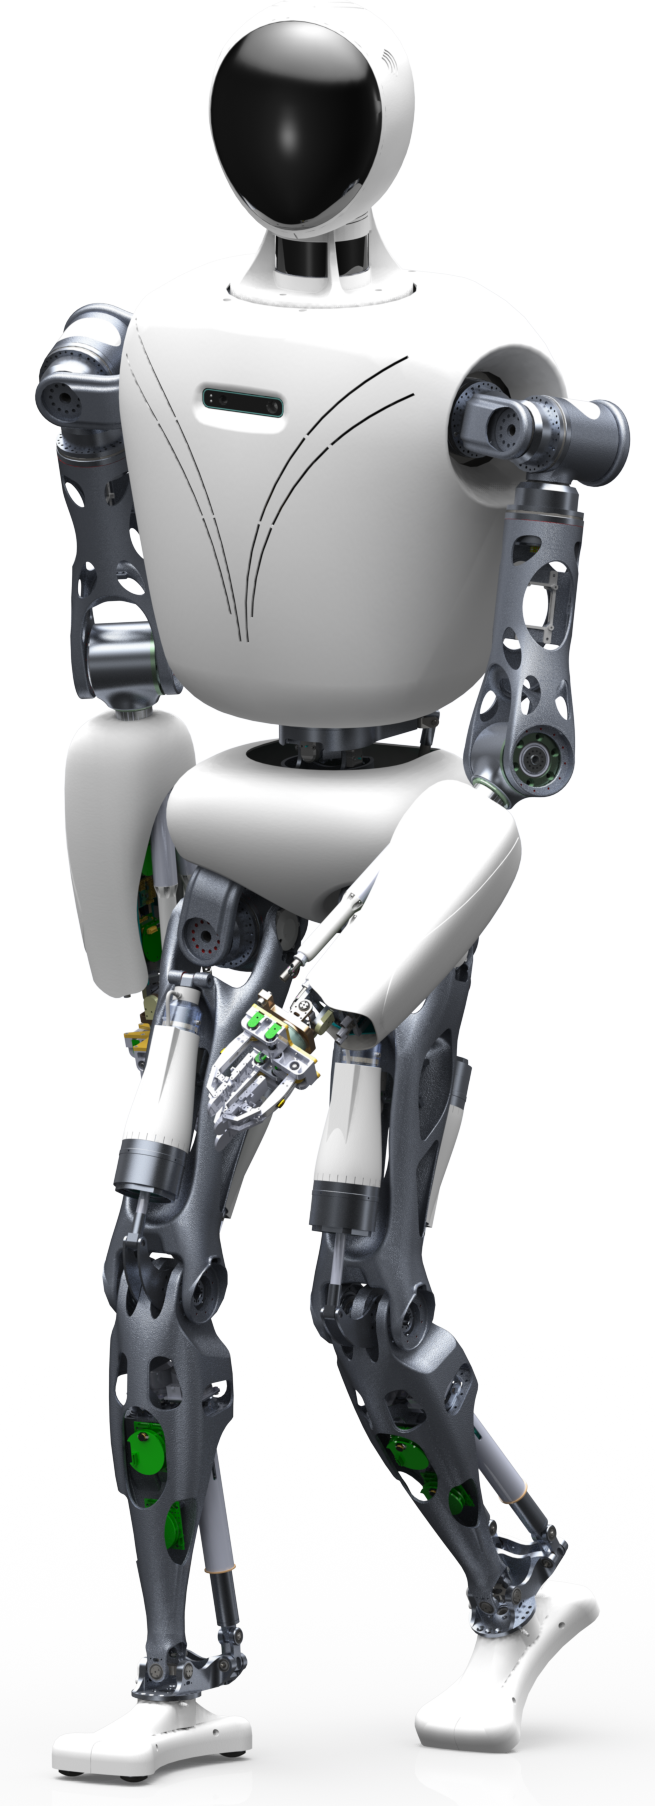
\includegraphics[width=.3\textwidth]{img/rh5_robot.png}
\caption{The recently presented RH5 is a lightweight and biologically inspired humanoid used as experimental platform within this thesis.}
\label{img:rh5_robot}
\end{figure} 

% Add to Appendix: 
% - Gelenkwinkel
% - Gelenkachsen Darstellung
% - URDF (abstract and full)
